%%% eval: (setenv "LANG" "de_DE.UTF-8")
% !TeX spellcheck = da_DK
% !TeX program = lualatex
\documentclass[12pt,fleqn,]{article}

\usepackage[danish]{babel}
\usepackage{../../../report/texfiles/SpeedyGonzales}
\usepackage{../../../report/texfiles/MediocreMike}
\usepackage{pdfpages}
\usepackage[contentBlocks]{markdown}
\title{Projektbeskrivelse til løsning af Rubiks terning med reinforcement learning}
\author{Søren Winkel Holm, Anne Agathe Pedersen og Asger Laurits Schultz\\
s183911, s174300, s183912}
\date{\today}

\fancypagestyle{plain}
{
	\fancyhf{}
	\rfoot{Side \thepage{} af \pageref{LastPage}}
	\renewcommand{\headrulewidth}{0pt}
}
\pagestyle{fancy}
\fancyhf{}
\lhead{}
\chead{}
\rhead{}
\rfoot{Side \thepage{} af \pageref{LastPage}}

\graphicspath{{Billeder/}}
\linespread{1.15} 

\begin{document}

\maketitle
\noindent
Rubiks terning er et eksempel på et diskret kombinatorisk problem med et utroligt stort tilstandsrum på $4.33\times 10^{19}$ distinkte, lovlige konfigurationer og kun én løsning. 
Projektet vil forsøge at løse dette problem eller dele af det ved hjælp af reinforcement learning. 

Den nyeste litteratur har formået at løse terningen til alle prøvede konfigurationer ved at kombinere dyb læring med approksimativ værdiiteration og vægtet A*-søgning\footnote{Agostinelli et al.: "Solving the Rubik’s cube with deep reinforcement learning and search", 2019 fra
	\url{https://www.nature.com/articles/s42256-019-0070-z}
}.
Intentionen med projektet er at forsøge selv at implementere dele af denne model. 
Med tid som en begrænsende faktor vil vi dog forsimple problemet, således at vi løser terningekonfigurationer, som kun er få skridt fra løsningen.
Derudover vil vi benytte gruppeteori til at beskrive udvalgte teoretiske aspekter af problemet.

I projektet ønsker vi at opnå, at
\begin{itemize}
	\item implementere en effektiv intern repræsentation af Rubiks terning
	\item analysere problemet og dets sværhed ved bl.a. brug af gruppeteoretisk repræsentation af terningens tilstande
	\item implementere Monte Carlo-træsøgning eller lignende på Rubiks terning
	\item implementere dyb Q-læring herunder et neuralt netværk med todelt struktur og eventuelt residuel arkitektur
	\item at samle træsøgningsmetoder og dyb Q-læring til at implementere model, der er baseret på DeepCube fra Agostinelli19
	\item at kunne løse lette terningekonfigurationer
	\item at kunne perspektivere problemet til anvendte diskrete optimeringsproblemer med store tilstandsrum som optimering af molekylstrukturer
\end{itemize}
I det følgende er vores egne læringsmål, diagrammer (projekt-lærred roteret er for læsbarhed; det er også vedhæftet seperat) og vores egen samarbejdskontrakt.
\newpage
\begin{markdown*}{hybrid}
/../læringsmål.md
\end{markdown*}




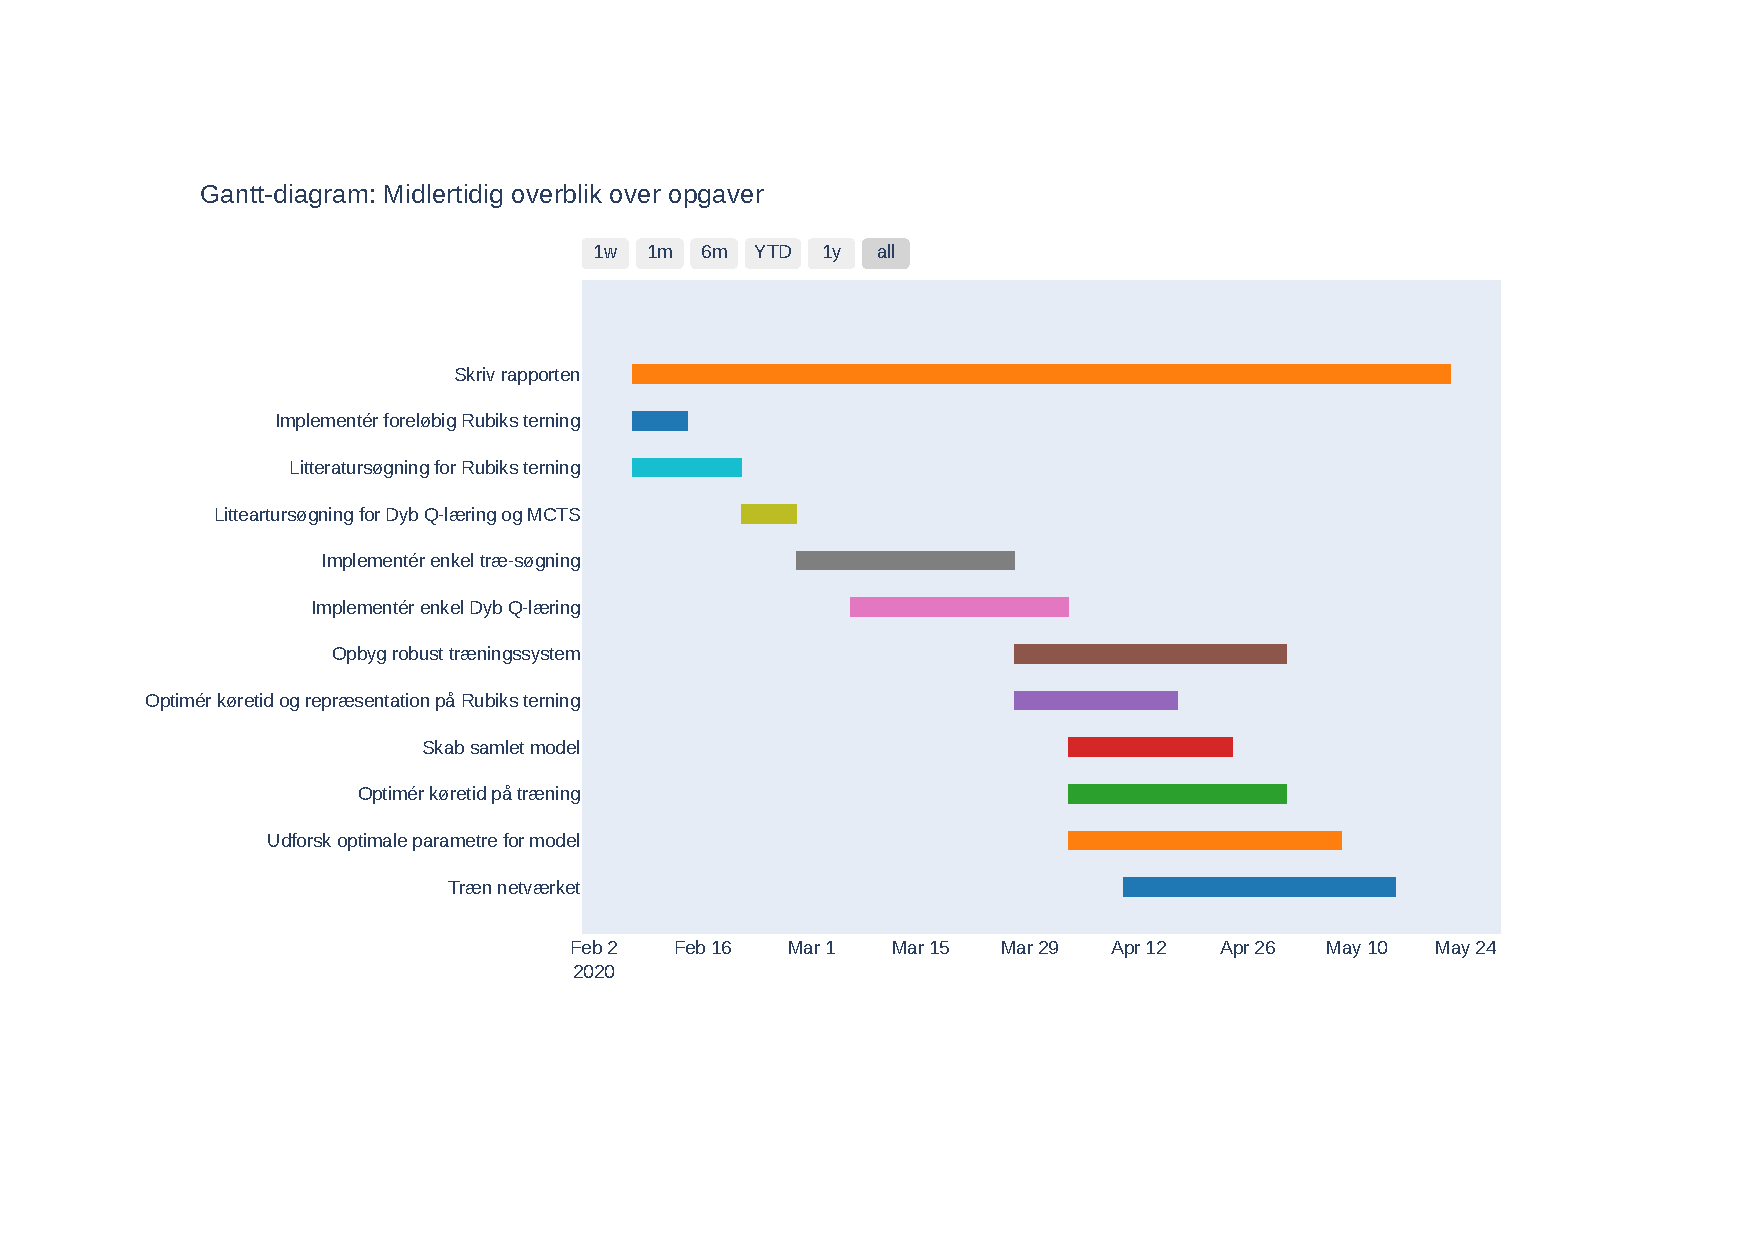
\includepdf{../gantt.pdf}
 

\begin{figure}[H]
	\centering
	\includegraphics[angle=90, width=\linewidth]{../project-canvas_udfyldt}
\end{figure}
\thispagestyle{empty}
\newpage 

\begin{markdown*}{hybrid}
/../samarbejdskontrakt.md
\end{markdown*}

\section{Underskrifter}
\begin{figure}[H]
	\centering
	\includegraphics[width=.5\textwidth]{sign_anne}\\
	\includegraphics[height=.5\textwidth, angle=90]{sign_asger}\\
	\includegraphics[width=.5\textwidth]{sign_soren}
\end{figure}

\end{document}

















